\documentclass{sigchi}

% Arabic page numbers for submission. 
% Remove this line to eliminate page numbers for the camera ready copy
%\pagenumbering{arabic}


% Load basic packages
\usepackage{balance}  % to better equalize the last page
\usepackage{graphics} % for EPS, load graphicx instead
\usepackage{times}    % comment if you want LaTeX's default font
\usepackage{url}      % llt: nicely formatted URLs
\usepackage{xcolor}
\newcommand\todo[1]{\textcolor{red}{#1}}

% llt: Define a global style for URLs, rather that the default one
\makeatletter
\def\url@leostyle{%
  \@ifundefined{selectfont}{\def\UrlFont{\sf}}{\def\UrlFont{\small\bf\ttfamily}}}
\makeatother
\urlstyle{leo}


% To make various LaTeX processors do the right thing with page size.
\def\pprw{8.5in}
\def\pprh{11in}
\special{papersize=\pprw,\pprh}
\setlength{\paperwidth}{\pprw}
\setlength{\paperheight}{\pprh}
\setlength{\pdfpagewidth}{\pprw}
\setlength{\pdfpageheight}{\pprh}

% Make sure hyperref comes last of your loaded packages, 
% to give it a fighting chance of not being over-written, 
% since its job is to redefine many LaTeX commands.
\usepackage[pdftex]{hyperref}
\hypersetup{
pdftitle={SIGCHI Conference Proceedings Format},
pdfauthor={LaTeX},
pdfkeywords={SIGCHI, proceedings, archival format},
bookmarksnumbered,
pdfstartview={FitH},
colorlinks,
citecolor=black,
filecolor=black,
linkcolor=black,
urlcolor=black,
breaklinks=true,
}

% create a shortcut to typeset table headings
\newcommand\tabhead[1]{\small\textbf{#1}}


% End of preamble. Here it comes the document.
\begin{document}

\title{Situated Display in Hospital Ward}

\numberofauthors{3}
\author{
  \alignauthor Ivan Naumovski\\
    \affaddr{ITU}\\
    \affaddr{Rued Langaardsvej 7, 2300 Copenhagen}\\
    \email{inau@itu.dk}
  \alignauthor Martino Secchi\\
    \affaddr{ITU}\\
    \affaddr{Rued Langaardsvej 7, 2300 Copenhagen}\\
    \email{msec@itu.dk}
  \alignauthor Diem Hoang Nguyen\\
    \affaddr{ITU}\\
    \affaddr{Rued Langaardsvej 7, 2300 Copenhagen}\\
    \email{hong@itu.dk}
}

\maketitle

\begin{abstract}
\textit{Etnographic studies of surgeons and their workflows show that issues exist such as information sharing between physians and the danger of spreading bacteria jjust to mention a few.
This journal attempts to solve some of the issues discovered in these studies.
A system that supports the workflow namely avoiding the spread of bacteria via touchless interaction has been designed.
To build the system multiple areas have been investigated, areas such as hardware prototyping, machine learning and software development.
This resulted in a system with 4 tiers, one handling data collection, another handling communication, a third one doing pattern recognition and the last one for presentation.
The system has quite a high recognition rate, due to some of the design choices taken.
For detailed information refer to the respective areas within the journal.
}
\end{abstract}

\keywords{
	Guides; instructions; author's kit; conference publications;
	keywords should be separated by a semi-colon.
	\textcolor{red}{Mandatory section to be included in your final version.}
}

\category{H.5.2.}{Information Interfaces and Presentation}{Input devices and strategies}
\category{I.2.6.}{Artificial Intelligence}{Learning}

See: \url{http://www.acm.org/about/class/1998/}
for more information and the full list of ACM classifiers
and descriptors. 

\section{Introduction}
Since the dawn of the computer age modalities have been an important aspect
to consider when interfacing with the machines, whether it has been done using keystokes, audio-control or gestures.

It has always been of high relevance to push the limits for how we interact with technology, mainly to empower the individual.

Technology is supposed to make common tasks even easier to achieve. Consider the case of a physically disabled person being empowered by using an alternative modality such as voice control.
%We have pushed the boundaries for how interaction with a computer is done.

In our case the focus is to improve on how people in the healthcare sector interact with technology.
In the healthcare sector interaction can actually prove to have negative effects, particularly bacteria can be transferred.

One way to avoid spreading bacteria is by avoiding physical interaction with input devices.

This can result in less time spent scrubbing or rinsing as the likelihood for microbacteria being 
transfered via input devices is reduced.

Ultimately alternative modalities could provide employees within the sector a 
way to use native hand gestures to perform tasks such as interacting with x-ray images.


\section{Previous Work}
There exist alot of prior work within the field of HCI which is relevant to our solution.
The papers which influenced this project the most will be mentioned in following section.

\subsection{Alternative Modalities}
Prior work in regards to pattern recognition has been of high relevance to our solution.
bla bla bla bla

\subsection{Smart Machines}
Prior work in regards to pattern recognition has been of high relevance to our solution.
bla bla bla bla



\section{System}
The system we have designed consists of multiple parts,
one being a input device, another being a data processer, 
a third one being a communications service and the last one being a presenter.

\subsection{The Input Device}
Our motion tracking device(MTD) has been built in such a fashion that it resembles a wrist watch.
This form factor makes it rather compact.
Additionally a lot of people wear watches on a daily basis which makes the device of a recognizable morphology and barely noticeable for people accustomed to such devices.
The MTD contains a list of components, the most important are 6DoF Sensor, Bluetooth and the Arduino microcontroller.

The \textbf{6DoF Sensor} is the heart of the device.
It is a board which contains an accelerometer and a gyroscope.
This means that it is possible to measure movement and rotation of the wrist of anyone wearing the device.
The sensor produces a set of 6 values: 3 for acceleration and 3 for rotation, each representing information on the axes of the coordinate system.
The input received from the 6DoF sensor is then propagated to the \textbf{arduino microcontroller}.
The arduino prepares the raw  values into JSON data. The JSON is then sent using the bluetooth device.

\begin{figure}[!h]
\centering
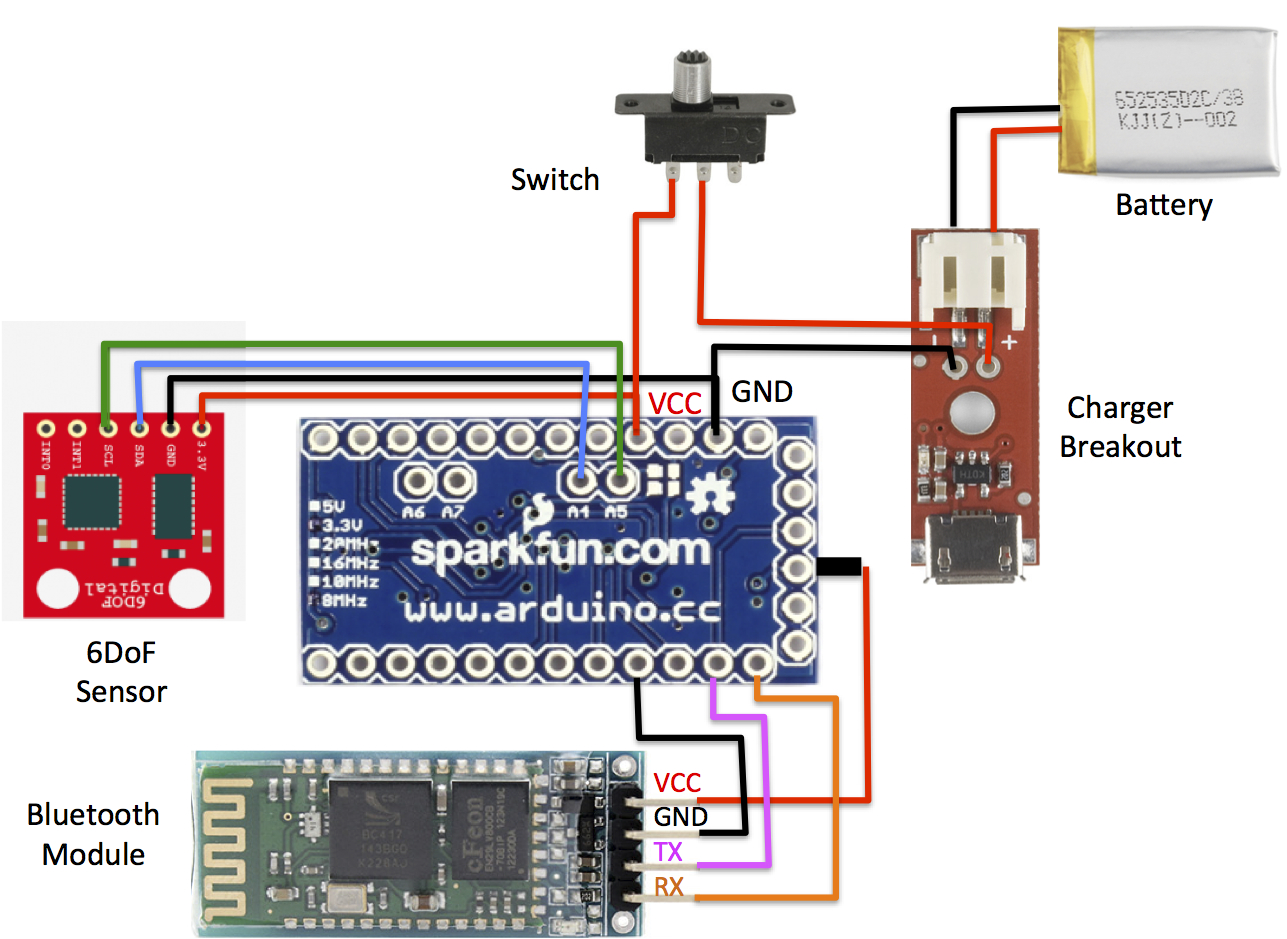
\includegraphics[width=0.9\columnwidth]{img/device_schematic}
\caption{This schematic shows the circuitry on the device.}
\label{fig:figure1}
\end{figure}

\subsection{Weka Gesture Recognition System}
Since the input device we have built is quite lightweight, data processing needs to be done elsewhere.
This provided us with the challenge of transferring data from one bluetooth capable device to another.
All the processing and preprocessing of the device's data is performed on a desktop application on a 
computer connected to the device.
Especially challenging was to find and use Java libraries that would allow to establish a Bluetooth 
connection with the device and to exchange data with the desktop application that would process it. 
For further technical details about the challenges encountered please refer to the Discussion section. 
\todo{add technical details about the rxtx fucking everything up}
Once the acceleration and rotation data is sent from the device to the computer,
 the values are smoothed with an average of the 20 previous values in order to avoid and reduce the effect of noise on the sensors.
 This phase is called preprocessing of the data. 
 This allowed us to have more precise information, as can be deducted from \textbf{Figure 2} and \textbf{Figure 3}

\begin{figure}[!h]
\centering
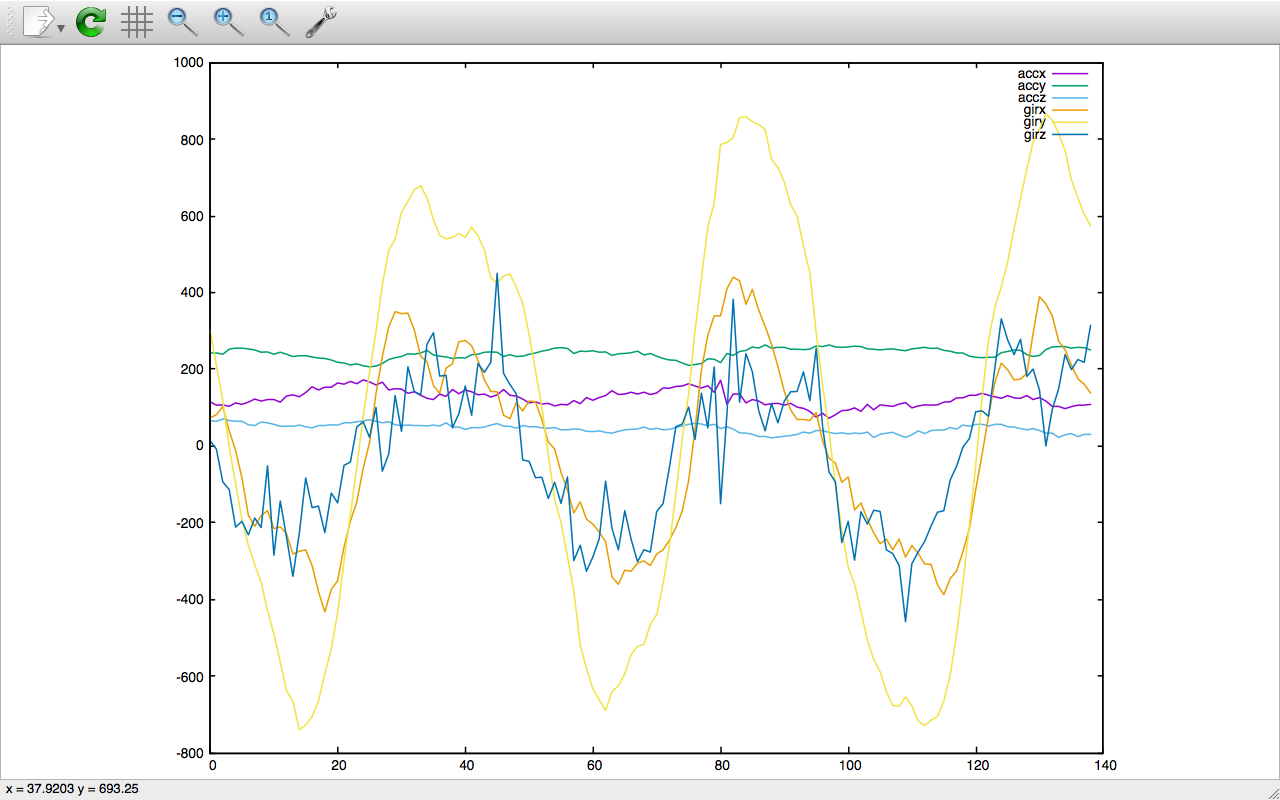
\includegraphics[width=0.9\columnwidth]{img/raw}
\caption{Data from the device before preprocessing.}
\label{fig:figure2}
\end{figure}

\begin{figure}[!h]
\centering
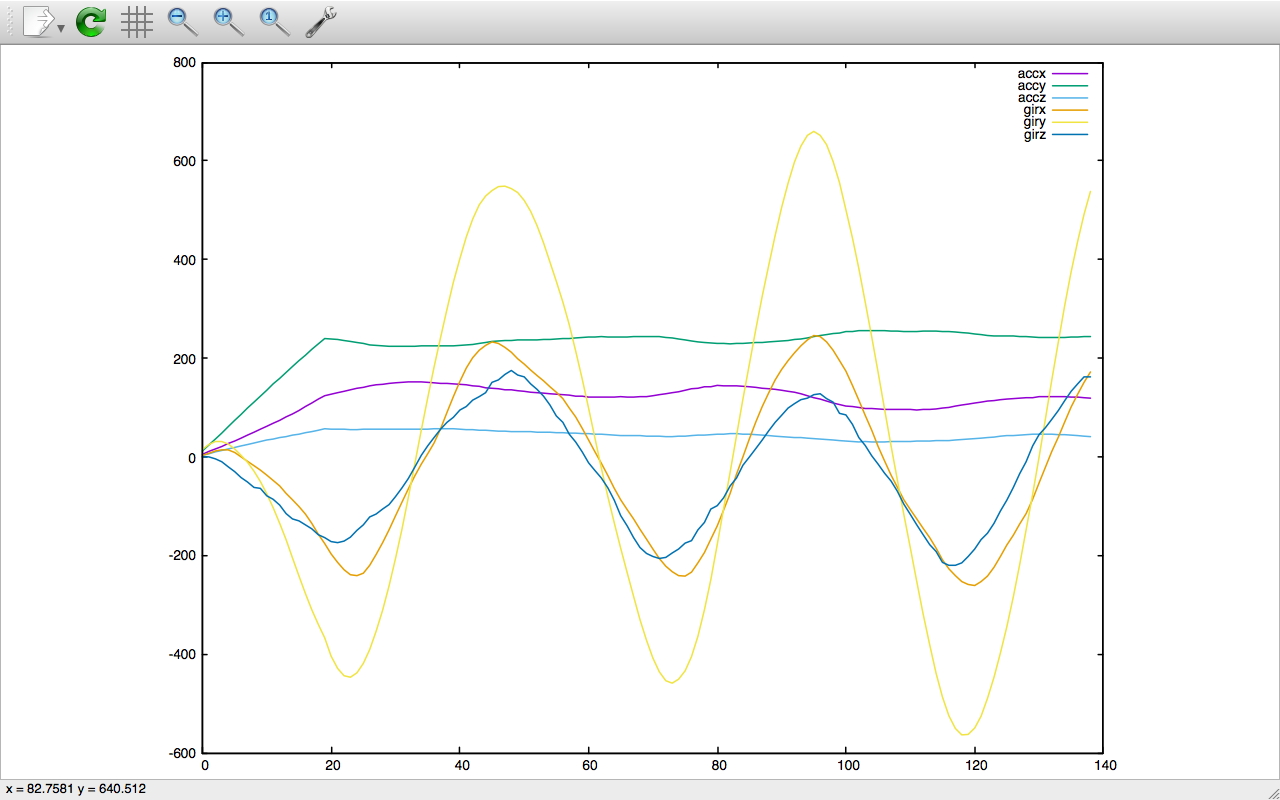
\includegraphics[width=0.9\columnwidth]{img/20}
\caption{Data from the device after preprocessing.}
\label{fig:figure3}
\end{figure}

For the actual processing and gesture recognition, we organized known gestures in a large training set, each individual gesture stored as a list of 50 * 6 values plus an identifier. 
We use Weka 3.6 to evaluate newly received data using a BayesNet classifier and comparing it to the training set.
The evaluation of the gesture is performed every 10 * 6 new values received.

\subsection{Android Application}
The android system is a quite limited system.
It is able to display  an image.
It provides the user with the possibility of panning and zooming a given image.
When the user zooms all the way out panning provides additional functionality.
Pannning left and right will then swap images from the set of loaded images.
\todo{add some user scenarios - images etc.}


\subsection{Webservice}
The communication between the Weka Gesture Recognition System and the Android Application is done by a simple webservice.
It provides GET, POST and DELETE requests which manipulate a queue.

GET pops all the queued gesture recognitions, 
POST pushes a new one to the service and DELETE clears the queue.

\begin{figure}[!h]
\centering
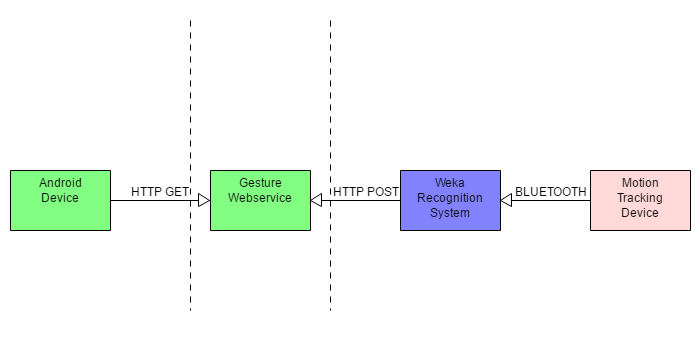
\includegraphics[width=0.9\columnwidth]{img/system_diagram}
\caption{This schematic shows the system interactions.}
\label{fig:figure4}
\end{figure}

\section{Result}
\section{Result}
The system sometimes encounters bluetooth interference from other devices which
cause the system not to work properly. Moreover, the weak Wi-Fi signals made system delays when simulating the hand gestures. 


\section{Discussion}

One of the less performant aspects of the project was the bluetooth connection, which was very unstable. 
We account interference in the ITU building mostly responsible for that. \todo{other reasons?}

\section{Acknowledgments}
We thank CHI, PDC and CSCW volunteers, and all publications support
and staff, who wrote and provided helpful comments on previous
versions of this document.  Some of the references cited in this paper
are included for illustrative purposes only.  \textbf{Don't forget
to acknowledge funding sources as well}, so you don't wind up
having to correct it later.

\section{References}

% Balancing columns in a ref list is a bit of a pain because you
% either use a hack like flushend or balance, or manually insert
% a column break.  http://www.tex.ac.uk/cgi-bin/texfaq2html?label=balance
% multicols doesn't work because we're already in two-column mode,
% and flushend isn't awesome, so I choose balance.  See this
% for more info: http://cs.brown.edu/system/software/latex/doc/balance.pdf
%
% Note that in a perfect world balance wants to be in the first
% column of the last page.
%
% If balance doesn't work for you, you can remove that and
% hard-code a column break into the bbl file right before you
% submit:
%
% http://stackoverflow.com/questions/2149854/how-to-manually-equalize-columns-
% in-an-ieee-paper-if-using-bibtex
%
% Or, just remove \balance and give up on balancing the last page.
%
\balance

% If you want to use smaller typesetting for the reference list,
% uncomment the following line:
% \small
\bibliographystyle{acm-sigchi}
\bibliography{ubicomp}
\end{document}
